% TODO change this uglyness
\chapter{The Serial Replication in \ak\ }

In this chapter we explain the machinery behind the serial replication in \ak\ and the role of synchronisers in it.
%TODO
%First of all, the semantics of AstraKahn on the TPL is described in terms of structures put in place for the coordinator, i.e. a controlling agent, or indeed a group of agents, responsible for progress and communication of the KPN vertices.
%
%The rest of the chapter is organised as follows. In sections \ref{ffp} and \ref{rfp} we explain why both cases are relevant to synchroniser analysis and give formal definitions. In section \ref{ffp_discussion} we discuss the original approach to the output of the infinite chain of replicas and in section \ref{approach} we propose another one. In section \ref{fp_detect} we provide detection algoritms for both cases.


    \section{\ak\ Approach to the Serial Replication}
The serial replication combinator creates conceptually infinite number of copies of its operand network, and connects them in a chain. Replication is demand-driven, hence replicas are created dynamically in runtime. A fresh replica is \emph{inactive}\footnote{More generally, we call a replica inactive when all of its synchronisers are in their start states, none of its channels has messages in them and no box is running}, hence it does not necessarily require significant resouces since \ak\ boxes are stateless and synchronisers require no resouces in their start state\footnote{When a synchroniser transitions back to the start state, it flushes its store variables}. Indeed the cost of replication is only felt when the replicas are active, which is the case when the first message is received until all messages have left the replica and all its synchronisers have returned to their start states.

In S-Net, the output from the replication pipeline is based on the record subtyping in the type system. The replication combinators in S-Net require the programmer to specify a termination pattern, so that each record that is a subtype of this pattern leaves the replication pipeline throught the output stream. In \ak\, a message leaves the replication pipeline exclusively via a special complement channel that is wired to the rest of the \ak\ network. The programmer has to make sure that the messages to be sent on are detected within the operand network and sent to this channel. \ak\ compiler recognizes the use of complement channels and provides the runtime support for them. Thus, the serial replication in \ak\ enforces a topological property of the operand network that is formally defined as follows. Consider the serial replication $N^{*}$ of an operand network $N$ with the input and output channel sets $\mathcal{I}$ and $\mathcal{O}$ respectively. Consequently, the set of matched inputs and outputs is $\mathcal{M}(\mathcal{I}, \: \mathcal{O}) = \mathcal{I} \cap \mathcal{O}$. In order for the serial replication $N^{*}$ to be able to produce output to the channel $x \in \mathcal{M}(\mathcal{I}, \: \mathcal{O})$, at least one box or a synchroniser in $N$ must have the output port wired to the complement channel $x'$.

The serial replication implementation in the \ak\ runtime system depends on the primitives the runtime system provides for the network construction. We briefly describe two approaches to the serial replication implementation with respect to the available primitives.

The first approach relies on a port wiring primitive $P$ that transmits messages immediately from one port to another without storing them. The serial replication network $A^{*}$ in \ref{fig:ffp_new} has the single input and the single output ports both named $x$. The operand network $A$ has the output port $x$ for the messages that proceed to the input channel of the next replica $A$ in the chain and the output port $x'$ for the messages that are supposed to leave the replication pipeline. During the compilation, the \ak\ compiler detects the use of the complement port $x'$ and encapsulates $A$ into the special network $N$ it as shown in Fig. \ref{fig:ffp_new}. The network $N$ inherits all the ports from $A$ and adds a corresponding input port $x'$. The input and output ports $x'$ in $N$ are connected with the wiring primitive $P$. The consequent replicas of $N$ are wired with the channels $x$ and $x'$.
\begin{figure}[h!]
\centering
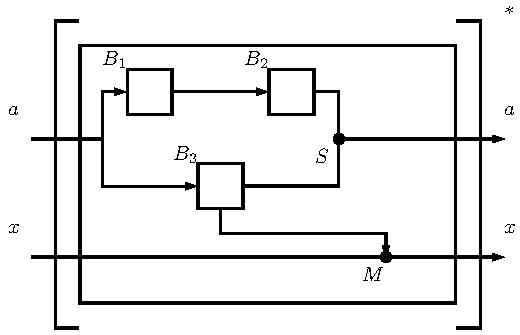
\includegraphics[scale=0.8]{figs/chapter_04_ffp_new.pdf}
\caption{The first approach to the serial replication $A^{*}$ implementation}
\label{fig:ffp_new}
\end{figure}
A message that $A$ sends to the output port $x'$ of $N$ cascades through all the active replicas. Once it has reached an inactive replica, the $A^{*}$ output channel $x$ is dynamically wired to the output port $x'$ of the last active replica of $N$. When the replica becomes active, the port $x'$ is rewired with the input port of this replica.

The second approach to the serial replication implementation relies on the merger with variable number of inputs. 




%\ak\ provides a termination mechanism that does not require to explicitly specify termination rules in the \ak\ application code. This mechanism is based on the concept of a fixed point.
%
%In mathematics, a fixed point of a function is an element of the function's domain that is mapped to itself by the function. Mapping this definition to messages and components we obtain the fixpoint definition of an \ak\ net: a message that leaves a net inactive after it was processed is called a fixpoint of the given \ak\ net. (NOT TRUE, FIX)
%
%TODO!! Explain that synchroniser analysis is relevant to fix-point resolution
%In order to utilize the fixed point the \ak\ compiler must be able to detect it. Due to separation of concerns \ak\ does not have to analyse the box code\footnote{except for CAL passport generation}, therefore the fixed point must be defined in synchronisers or the network topology of a net. It means that the net graph must have at least one path that goes exclusively via synchronisers (TODO fix) or straight through the net without traversing any box.
%
%\ak\ defines two types of a fixed point: a forward fixed point and a reverse fixed point. The intention of a forward fixed point is to cut infinite tail of inactive replicas chain. The reverse fixed point is an optimisation of an input connection that has to cascade through the chain to a replica that is ready to accept the data. Its intention is to bypass the replicas that transmit messages without change (TODO not good). Later we will see that a replica does not have to be inactive in order to that.
%
%With the reference to fixed point utilisation we will call the \ak\ replication operator the fixed point series (FPS).



    \section{Forward Fixed Point Series\label{ffp}}
In this section we provide the original approach to the forward fixed point.


Consider a vertex $v$ that has an input and an output channel, both named $x$.

\begin{definition}The vertex $v$ is said to have a forward fixed point in $x$ if and only if the following requirements are satisfied:

\begin{enumerate}
\item There exists a condition $p(m)$ on the content of the message $m$ received by the vertex on the input channel $x$ under which it follows a unique non-branching path to the output channel $x$ without traversing any boxes.

\item The path can traverse synchronisers, but then whenever $p(m)$ is true and the synchroniser is in the start state, it must accept $m$ and transition back to the start state while sending the message $m$ on the path unchanged and without producing any other output.

\end{enumerate}
\end{definition}

% Give a definition for "edge that satisfies the fixed-point definition"
The condition $p(m)$ may not be unique for each vertex, and when it is not, a disjunction of all such conditions is called the fixed-point condition of the vertex on channel $x$. The condition can also be a tautology, in which case the forward fixed point is called unconditional. When the path traverses several vertices, the fixed-point condition is a conjunction of their fixed-point conditions.

% Draw a picture to explain conj and disj
  \begin{figure}[h!]
  \centering
  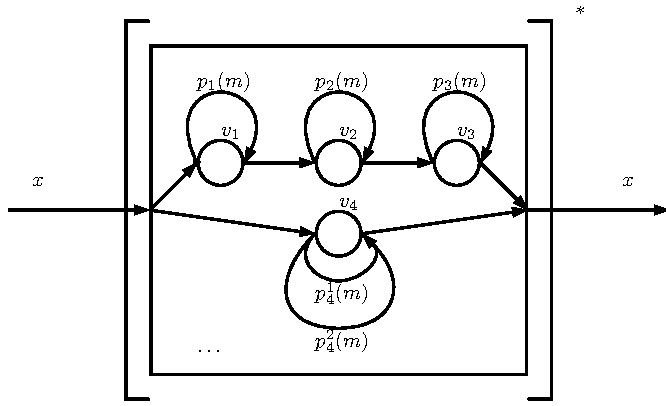
\includegraphics{figs/chapter_04_ffp.pdf}
  \caption{Forming of the forward fixed-point condition of a vertex.}
  \label{fig:ffp}
  \end{figure}

A replicated vertex in Fig. \ref{fig:ffp} is a net that has a unique path $[v_1, \: v_2, \: v_3]$ that traverses only synchronisers. The synchroniser $v_2$ has two edges that loop around the start state and satisfy the fix-point definition (TODO fix; explain how). The firing conditions for those edges are $p^{1}_2(m)$ and $p^{1}_2(m)$. A message $m$ is a fixed-point when it satisties any of them, i.e. $p^{1}_2(m) \lor p^{1}_2(m)$. The synchronisers $v_1$ and $v_3$ have fixed-point conditions $p_1(m)$ and $p_3(m)$ respectively, where $p_i(m) = p^{1}_i(m) \lor \dots p^{j}_i$, $i=1,3$ and $j$ is the number of edges that satisfy the fixed-point definition (TODO fix). Then the fixed-point condition of the whole net is $p_1(m) \land (p^{1}_2(m) \lor p^{1}_2(m)) \land p_3(m)$.


%Forward fix point puts some requirements on the message value and not its type.

%Forward fix point checker checks if a message satisfies a set of requirements to be a fix point.

%Forward fix point checker is a code generated from the synchronisers source code. It utilises message api like fuction that tells that a message has variant $v$ etc.


    \subsubsection{Output from the Forward FPS}
In this section we will clarify how the FPS is wired to the rest of network and how the output of the FPS is produced.

Strictly the FPS is not a connection since it does not simply wire the replicas of its component. It also creates a set of output channels and in some cases augments the replicas with some auxiliary vertices. However, in the main it wires the replicas in a serian fashion and we will consequently call the FPS a connection.

We denote the FPS connection as $A^{*} = A' \: .. \: A' \: .. \: A' \: .. \: \dots$, where $A'$ is the network that contains $A$ and provides additional wiring to ensure that all output channels of $A'$ match its input channels bijectively.

The FPS connection $A^{*}$ defines the output channel set $\mathcal{N}_{out}$ as follows:
\begin{equation}
\mathcal{N}_{out} = \{ name(c) \: | \: c \in \mathcal{O} \land fp(c) \}\nonumber
\end{equation}
where $\mathcal{O}$ is the output channel set of $A$ and the predicate $fp(c)$ is true on any channel $c$ that has a forward fixed point. The FPS creates a set of fresh output channels $\mathcal{O}^{*}$ taking the names from the set $\mathcal{N}_{out}$. A message coming to an inactive replica on any channel $c$ with $name(c) \in \mathcal{N}_{out}$ and which satisfies the fixed-point condition on that channel is immediately transferred to the identically named output channel from $\mathcal{O}^{*}$.

  \begin{figure}[h!]
  \centering
  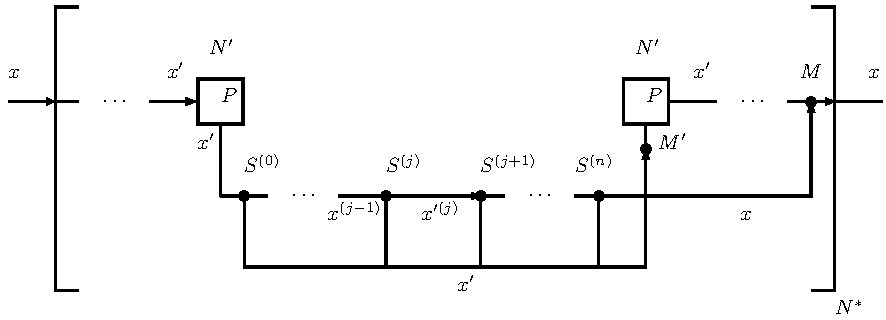
\includegraphics{figs/chapter_04_ffp_out.pdf}
  \caption{Output from the forward fixed-point series.}
  \label{fig:ffp_out}
  \end{figure}

In Fig. \ref{fig:ffp_out} a replicated vertex $A$ has the fixed-point condition $p(m)$. Synchroniser $S_f$ is inserted before every inactive replica $A'^{(i+1)}$ to check whether a message in channel $a_{i}$ satisfies the condition $p(m)$. If $p(m)$ is satisfied, the message $m$ is sent to the output channel $a$ of $A^{*}$. Otherwise, it is sent to the input channel $a^{(i+1)}$ of the next replica. The listing of the synchroniser $S_f$ is given in Fig. \ref{ffp:synch_filt}.

\begin{figure}[h!]
\begin{lstlisting}[frame=single,mathescape]
synch $S_f$ ($a_i$ | $a_{i+1}$, $a$)
{
  start {
    on:
      $a_{i}$.$p(m)$ {
        send this => $a$;
      }
      $a$.else {
        send this => $a_{i+1}$;
      }
  }
}
\end{lstlisting}
\caption{The synchroniser $S_f$}
\label{ffp:synch_filt}
\end{figure}

The merger $M$ accepts input messages from all synchronisers $S_f$ that are inserted before inactive replicas of $A$ (TODO fix) and sends the messages to the output channel $a$.


%An FPS is a form of replication wiring whereby an infinite chain of replicas is created, connected in series. The connection is denoted as A* for any operand network A and can be thought of as the equivalent of $A^{*} = A'..A'..A'.. \dots$ where $A'$, called the streamlining of the vertex A, is a network that contains A and provides some additional wiring to ensure that each output channel of A? matches an input channel and vice versa. We will dwell on the streamlining procedure a little further down, and at this point only remark that if all output channels of A match its input channels bijectively, A' = A.



    \subsection{Discussion\label{ffp_discussion}}
%Why is the path required to be unique?
The definition of the forward fixed point required the uniqueness of the fixed point path. (TODO) Explain why it is required to be unique.

%Why does it consider only the start state? Why can't it be a closed subset of states in a general case?
%Explain that it should be ok but it makes the approach really bad (because need to add the sane edge to every state in the closed set)
The forward fixed point definition requires the traversed synchronisers to be in their start states when a message that satisfies the fixed-point condition is received. This requirement does not mean that synchronisers have to stay in their start states. A net in Fig. \ref{fig:ffp_net} demonstrates such behaviour. The synchroniser $S$ that implements the fixed-point condition $p(m)$ on channel $a$ moves to the state $s_1$ when it received a message from channel $b$. A message received from channel $c$ make $S$ move from state $s_1$ to the start state. The synchroniser $S$ can implement some processing of messages from channels $b$ and $c$, i.g. pattern matching, combining and sending to the output channels. However, to make sure that $S$ is in the start state when a message from channel $a$ is received, messages need to be ordered so that a message from channel $a$ always arrives before a message from channel $b$ and a message from channel $c$. Such ordering can be implemented with a synchroniser. In Fig. \ref{fig:ffp_net} this synchroniser is denoted $Ord$.

  \begin{figure}[h!]
  \centering
  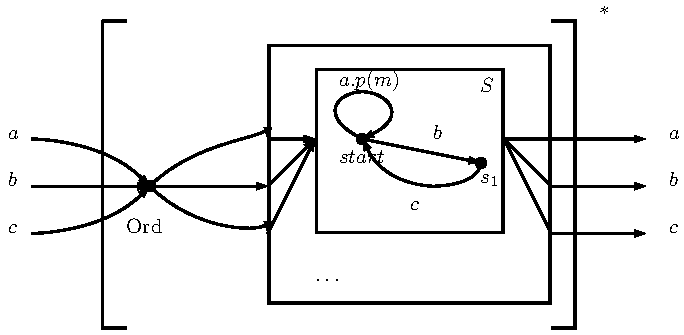
\includegraphics{figs/chapter_04_ffp_net.pdf}
  \caption{An example net where the fixed point synchroniser does not have to stay in its start state}
  \label{fig:ffp_net}
  \end{figure}

Synchroniser $S$ has a subset of states $s=\{start, \: s_1\}$ and both states $start$ and $s_1$ read messages from other channels $b$ or $c$, however, no transition to a state outside of the subset $s$ exists. Addition of a fixed-point edge to state $s_1$ could potentially let messages from channel $a$ that satisty the fixed point condition leave the replication pipeline earlier. This idea is generalised as follows: the fixed-point synchroniser can have a subset of states that have the fixed-point edge, and the synchroniser may still be sensitive to other input channels, as long as it does not cause a transition to a state outside of the subset. Thus, the definition of the forward fixed point should be extended to cover the described case.

The extended approach makes the maintenance of the fixed-point condition inconvenient because the programmer needs to keep track of changes in all fixed-point edges of synchronisers. Moreover, if the replicated vertex has several synchronisers on the fixed-point path, it may be hard to find and maintain the fixed-point condition at all. Considering these drawbacks, the question arises if the idea of terminating the processing of a message implicitly is good.

%And it creates dificulties for the synchroniser analysis that make it conservative. I.e. in some cases when the fix point exists the compiler may miss it.

The idea of the implicit processing termination originates in S-Net. In S-Net the termination could be done by its type system means: the record leaves the replication pipeline when all its fields are flow-inherited. However, it was implemented in a more explicit way: whether a record leaves the replication pipeline is decided by checking if the record matches the specified termination pattern.

%However, the final decision for fix-point resolution was made on the side of simplicity (????) TODO What is the solution in S-net??

In this chapter we propose a straightforward approach to the FPS. The fixed-point satisfaction check is now maintained in the box code. The box sends the fixed points to a special channel that goes through the replicated vertex without traversing any box or synchroniser. Messages that are sent to this channel leave the replication pipeline.

%Now the \ak\ compiler can check the fix-point out of the network topology because there's a channel connected to the box that.



    \subsection{Forward Fixed Point Detection\label{ffp_detect}}
The approch we proposed in section \ref{approach} makes the forward fixed-point detection trivial. The forward fixed-point detection does not require synchroniser analysis anymore. The \ak\ compiler just checks that the forward fixed-point exists in the network topology.

We split the forward fixed-point detection problem into the following subproblems:
\begin{itemize}
\item Choose a data structure to represent a net
\item Provide an algoritm for the fixed-point path detection
\item Provide an algoritm for recursive fixed-point check
\end{itemize}

%% Provide detection algorithm

\ak\ compiler needs to just detect the forward fixpoint from the network topology (answer 'yes' or 'no' if the fixpoint exists). If the fixpoint was not found then the network is infinite and inconsistent.

Forward fixpoint detection is pure network topology analysis. Find a way in a net graph that goes exclusively through mergers and some other vertex output to this channel.

How to represent the net graph.
We have (at least) 4 types of vertices: boxes, synchronisers, nets, mergers.
If we find net on the way we have to run the analysis for it (recursively). For example:
% A net in wrapped in a Star combinator
%  __                               __
% |       _____________________       | *
% |      |    __      __       |      |
% |     _|  /|__|----|__|-\    |_     |
% |  a |_|-|      __      |----|_| a  |
% |      |  \----|__|-----/    |      |
% |     _|                |    |_     |
% |  b |_|---------------|N|---|_| b  |  - fix point channel b (goes straight throuhg the net)
% |      |               net   |      |
% |      |_____________________|      |
% |__                               __|
%
We could represent the net graph as a multigraph (where a vertex, which is a box, a synch, a net or a merger can have several inputs and several outputs).
But it is inconvenient because we cannot specify the connections to the net inputs and outputs. In order to specify this connections, we can have ports as vertices of a graph.

We assume that the ports graph is a connected graph.

We can filter the subgraph those vertices are only mergers and nets. In this case with the assumption of the original graph connectivity, the resulting graph is a connected graph by construction.
We construct this graph by traversing all the vertices from the 'start' vertex (we have to keep it in the graph structure). We take the successors of the current vertex and check their 'type'. If the successor is a merger, we add it to the resulting graph and traverse it. (Anyway, generating such a graph seems useless since we can detect the paths we need with just a single traversal)

Or we can leave the graph as is and just put a condition of every vertex we visit that it must be net or merger.



    \section{Reverse Fixed Point Series\label{rfp}}
% TODO: I don't like the reason. Why was the reverse fixed point introduced?
% reverse fixed point is the basic optimisation that preserves growth of the replicas chain.
As the chain of replicas evolves, it may be the case that some replicas in the head of the chain are active yet they just transmit messages without a change. \ak\ is commited to detect such replicas and optimise the connection so that the data are sent directly to a replica that is ready to process it. 

%channels are ordered, need to insert synchronisers
In this section we provide the approach to the reverse fixed point.

Consider a vertex $v$ that has an input and an output channel, both named $x$.

\begin{definition} The vertex $v$ is said to have a reverse fixed point in $x$ if and only if the following statements hold:

\begin{enumerate}
\item A unique non-branching path from the input to the output channel $x$ exists that does not traverse any boxes.

\item Every synchroniser $S_i$ on the path has a subset of states, which we denote as $s_i$, such that in each of these states every message on the path is immediately transferred without being changed or even stored, causing the synchroniser to remain in the same state\footnote{It should also be borne in mind that the values of any state variables form a part of the synchroniser state}. In a state from $s_i$ the synchroniser $S_i$ may still be sensitive to other input channels, as long as this does not, under any circumstances, cause a transition to a state outside $s_i$.
\end{enumerate}
\end{definition}

The vertex $v$ is said to be in a reverse fixed point state on channel $x$ when each $S_i$ is in a state that belongs to its $s_i$.

%%%%%%%%%
%%  Motivation for the reverse fixpoint
%%%%%%%%%
The reverse fix-point is defined to unify backslash \ combinatior and the star in terms of their functionality, which was never done in S-Net(TODO which patterns??). The intention is that they only differ in the pressure propagation strategy. The backslash creates no pressure (TODO why??) in its looped channel, and the start mantains and propagates the pressure in channels between instanses.

% probably a picture
%
% backslash (* is the synchroniser)
%      _________
%    \|/ _____  |
% ____*_|     |_|
%       |_____|
%
%
% Star with the reverse fix point
%        __________________
%      _|___________       |
%    _|______       |      |
%   |    __ \|/ __ \|/ __ \|/ __
% --*---|__|-*-|__|-*-|__|-*-|__|-- ...
%

The reverse fix point is more the way to write code. It is the way to program a loop dependency, when the result of the iteration depends not only on the result of the previous iteration but on the new incoming data. The difference with backslash is in the pressure propagation.

If you want the feature, you must define a closed set of translating states in every synchroniser on the fp path.


\subsubsection{Rewiring of the Reverse FPS}
The reverse fixed point optimises an input connection that has to cascade through the chain to a replica that is ready to accept the data. Any input channel $x$ wired to an active replica $A_i$ that transitions to a reverse fixed point state on that channel is disconnected from $A_i$ and dynamically rewired to the input channel $x$ of the next replica on the chain $A'_{i+1}$.

%pic


    \subsection{Discussion}
Order of messages in the reverse fixed point may be changed, because a message may put the replica into the reverse fixed-point state and go for processing into this replica. In this case the messages that came to the replica that is in the reverse fixed-point state may overcome the message processed in the replica. This changes the order of messages. If the progrmmer wants to preserve the order, he must mind it. It may be fixed by creating a separate channel for RFP messages and putting a synchroniser that blockes the RFP channel while there's no message from the output channel (this is for operand network with one input channel, with two it can be more dificult if there're races between the channels that wire replicas).

The replication combinator is just a wiring pattern that does not have to guarantee race-safety. For example, if the operand network is not race-safe, the star is not race-safe as well.


    \subsection{Reverse Fixed Point Detection\label{rfp_detect}}
%%% Synch state conditions for the reverse fixpoint state
A message is not changed by the synchroniser in some state when:
- message is sent out by the synchroniser without any changes and storing in any transition including user-specified $else$ ($this$)

A message sent in autogenerated $else$ transition is disregarded by the synchroniser.

If a message is sent out in a user-defined $else$ then we have to make sure that the message get to this $else$. Before $else$ the channel may be tested for variants and segmantation marks, so we have to make sure that the message doesn't contain these variants/not a segmentation mark whatever.
%%%%%%


Choose any convenient structure for nets to resolve fix points. It may be a kind of graph that traversing it it's easy to find paths that only consist of synchronisers.
It could be a hypergraph (each vertex may have several inputs and several outputs) with type vertices (something that indicates whether vertex is a synchroniser or a box)

This chosen structure can be build in the net parser of from the net compiler internal data structure.

Then we need to represent a set of possible paths in this hypergraph that only contain synchronisers. And a traversal of the hypergraph to find all these paths.

Then we analyse every synchroniser in each path for the satisfiability of fix point conditions.

